\documentclass{article}

\usepackage{graphicx}
\usepackage{indentfirst}
\usepackage[czech]{babel}
\usepackage[utf8]{inputenc}
\usepackage{blindtext}
\usepackage{geometry}
\usepackage{lmodern}
\usepackage{titlesec}
\usepackage{wrapfig}

	\geometry{
	a4paper,
	%left=30mm,
	%right=30mm,
	%top=25mm,
	%bottom=35mm,
	headheight = 16pt ,
	marginparsep = 10pt,
	}
\marginparwidth \dimexpr \evensidemargin + 1in - \marginparsep - 40pt

%\parindent=1.2em
\renewcommand{\baselinestretch}{1.4}

\titleformat*{\section}{\LARGE\bfseries}
\titleformat*{\subsection}{\Large\bfseries}
\titleformat*{\subsubsection}{\large\bfseries}

\setlength{\parskip}{0pt plus 1pt}

\setlength{\parindent}{11.2pt}

\begin{document}
\begin{titlepage}
   %\begin{center}
%       \vspace*{1cm}
	
       %\begin{wrapfigure}{L}
       %		
\includegraphics[width=5cm\textwidth]{ctu_logo_black-1.png}
	%\end{wrapfigure}
            
	\begin{wrapfigure}{l}{0.3\linewidth}
	
\includegraphics[width=3cm]{ctu_logo_black-1.png}
	\end{wrapfigure}
	
	\large    
	\noindent
	\\   
       České vysoké učení technické v Praze\\
       Fakulta elektrotechnická\\
       8.4.2022
       \\ \\ \\ \\ \\ \\

	\begin{center}
	\huge
       \textbf{Obří slalom s Turtlebotem}

       \vspace{0.5cm}
       \Large
        Technická zpráva
            
       \vspace{1.2cm}

       {\bf Matouš Soldát, Šimon Soldát, Karolína Volfíková}

       \vfill
       
	\end{center}
%        \large
%       {\bf Vedoucí práce:} Ing. Radek Janča, Ph.D. \\
%       {\bf Konzultant:} Mgr. Jiří Hammer, Ph.D. \\
%       {\bf Obor:} Lékařská elektronika a bioinformatika \\
       
            
       %\vspace{0.8cm}
     
            

\end{titlepage}


%\title{Obří slalom s Turtlebotem, technická zpráva}

%\author{Matouš Soldát, Šimon Soldát, Karolína Volfíková}


\newpage

\tableofcontents

\newpage

\section{Úvod}
\subsection{Zadání úlohy}

	Cílem úlohy \uv{obří slalom} je projetí dráhy vyznačené tyčkami různých barev robotem. Dvojice stejně barevných tyček tvoří branku. Šířka jednotlivých branek je 450-600 mm a maximální vzdálenost středů dvou po sobě následujících branek je 1000 mm. 
	
	Na počátku úlohy je robot umístěn do startovní pozice. Jeho střed se nachází minimálně 300 mm a maximálně 1300 mm od startovní branky, kterou tvoří zelené tyčky, a jeho podélná osa s osou startovní branky nesvírá úhel větší než 60°. Minimální vzdálenost dvou tyček různých branek je 500 mm. Navíc směr jízdy může s osou branky svírat maximálně 30°. Na začátku je alespoň jedna z tyček startovní branky v zorném poli RGB kamery. Po průjezdu startovní brankou musí robot projet trať, na které se střídají modré a červené branky, aniž by se jich dotkl. Poslední branka není nijak definována a robot po jejím projetí může pokračovat v jízdě. 
	\\
	\\
	\\
	
	
\begin{figure}[h]
	\centering
	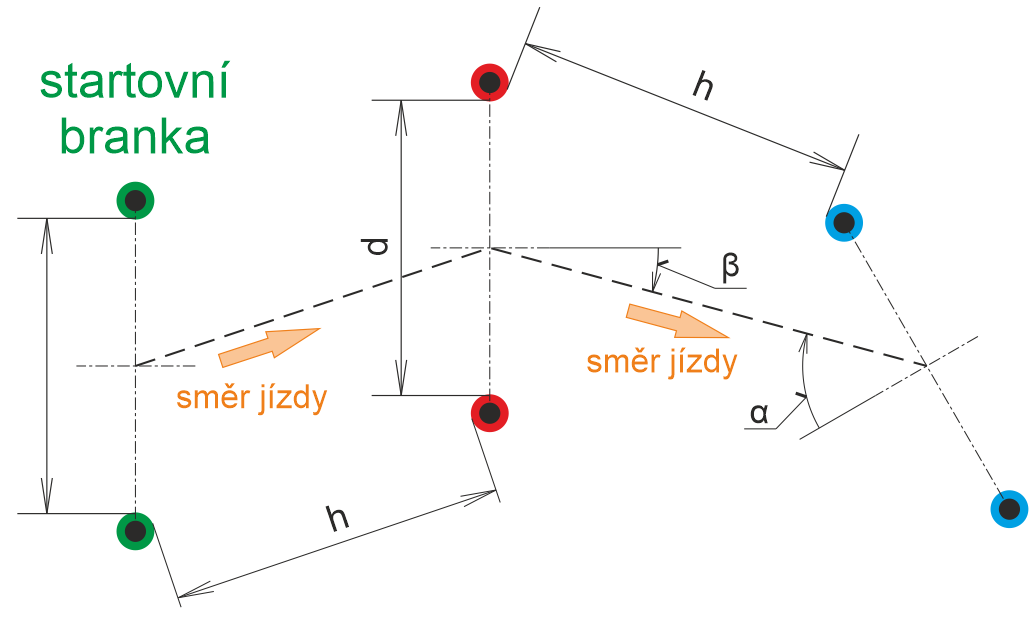
\includegraphics[width=10cm]{vykres_slalom_obri.png}
	\caption{Schéma dráhy obřího slalomu}
\end{figure}

\newpage

\subsection{Použitý robot}

	Pro řešení úlohy byl použit TutleBot 2. Jeho základnu tvoří zařízení Kobuki, které poskytuje základní funkční prvky: systém pro pohyb robotu, bumper, odometrii. Robot je ovládán přes NUC PC s frameworkem pro softwarový vývoj robotu ROS (Robot Operating System). Dále je na robotu umístěn jeden ze dvou RGBD senzorů: Orbex Astra (pro roboty s číslem 1, 2), Intel RealSense (pro roboty s číslem 3-7). % ? 
	\\
	\\
	\\
	
\begin{figure}[h]
	\centering
	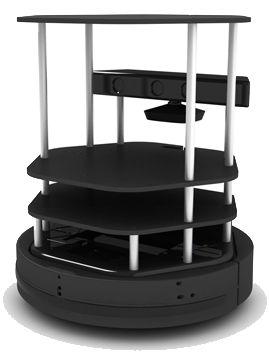
\includegraphics[width=5cm]{turtlebot_2.png}
	\caption{TurtleBot 2}
\end{figure}
	

\clearpage


\section{Řešení}

\subsection{Segmentace}
	
	Pro nalezení jednotlivých tyček v obraze získaném z RGB kamery jsme zvolili segmentační metodu prahování. Nejprve jsme získali obraz z kamery pomocí funkce {\it get\_rgb\_image()}. Převedli jsme obraz z RGB do HSV barevné reprezentace a zvolili optimální prahové hodnoty. Pro každou barvu jsme experimentálně nalezli práh tak, že jsme RGB kamerou pořídili několik snímků každé tyčky při různém osvětlení. 

\vspace{0.5cm}

\begin{table}[h]
\centering
\begin{tabular}{lllll}
\hline
\bf{Barva} & \bf{$H_{exp}$} & \bf{$H_{diff}$} & \bf{$S_{min}$} & \bf{$V_{min}$}\\
\hline
Zelená & 65 & 25 & 80 & 60 \\
\hline
Modrá & 100 & 25 & 230 & 80 \\
\hline
Červená & 2 & 8 & 150 & 70 \\
\hline

% H: stredni hodnota hue, ocekavana
% S: min
% V: min

\end{tabular}

\caption{Tabulka zvolených prahových hodnot, kde: $H_{exp}$ je střední hodnota odstínu, $H_{diff}$ je maximální povolený rozdíl měřené a střední hodnoty odstínu, $S_{min}$ je minimální saturace a $V_{min}$ minimální jas.}

\end{table}

\vspace{0.7cm}

	Dále jsme v obraze detekovali spojité oblasti jako kandidáty pro tyčky pomocí OpenCV funkce {\it connectedComponentsWithStats()}. Odstranění nežádoucích oblastí jsme realizovali pomocí výstupů této funkce -- definovali jsme minimální požadovanou plochu {\it S} a také podmínky pro poměr výšky {\it h} a šířky {\it w}:
	
\begin{equation}
	S > 2500 \; [px],
\end{equation}

\begin{equation}
	r = \frac{h}{w} = 5.1,
\end{equation}

\begin{equation}
	r_{diff} < 3,
\end{equation}
	kde $r_{diff}$ je rozdíl poměru měřených hodnot a definovaného poměru {\it r}. 

\subsection{Orientace v prostoru}

	Pro orientaci v prostoru jsme využili point cloud. Point cloud je sada bodů, které reprezentují daný objekt v prostoru. Každý bod je charakterizován souřadnicemi {\it x, y, z}. Point cloud získáme z funkce {\it get\_point\_cloud()} jako matici o velikosti 480 x 640 x 3. 
	
	Vektor třetí dimenze si uložíme jako {\bf z} a v matici jej nahradíme vektorem jedniček -- tím převedeme matici do homogenních souřadnic. Novou matici označíme jako {\bf $M1_{CAM}$}. Následně využijeme rovnici:

\begin{equation}
	{\bf X} = \lambda \cdot {\bf K^{-1}} \cdot {\bf M1_{CAM}},
\end{equation}
	kde ${\bf K^{-1}}$ je matice hloubkové kamery se souřadnicemi se středem v kameře získaná funkcí {\it get\_depth\_K()} a $\lambda$ je empiricky zjistěná hodnota. Pro její získání jsme provedli osm měření vzdáleností tyček od sebe s hodnotou $\lambda = 1$. Poté jsme na výsledky aplikovali metodu nejmenších čtverců a dostali hodnotu $\lambda = 429$. 
	
	Z matice {\bf X} opět odstraníme vektor třetí dimenze a nahradíme jej vektorem {\bf z}. Výsledná matice {\bf  $M_{CAM}$} je matice souřadnic se středem v robotu. 
	
	Při pohybu jsme využívali funkcí {\it reset\_odometry()} a {\it get\_odometry()}. {\it Reset\_odometry()} nastaví počátek souřadnic na aktuální pozici robotu. {\it Get\_odometry()} vrací relativní vzdálenost uraženou od posledního volání {\it reset\_odometry()}. 

\subsection{Pohyb na dráze}

	

	%Po spuštění robotu se aktivuje hledání zelené branky. Robot se otáčí, dokud nedetekuje obě zelené tyčky. Změří vzdálenost mezi nimi a najde střed branky. Otočí se o úhel $\alpha$ a rozjede se ve směru vektoru {\bf m}. Dojede až na osu branky, zastaví se a resetuje odometrii. Poté proběhne rotace souřadnic o úhel $\phi$, robot se o tento úhel otočí v opačném směru a rozjede se ve směru {\bf m}. 

	%Po tom, co robot projede startovní brankou, detekuje dvě nejbližší tyčky stejné barvy a stejným způsobem mezi nimi projede. 
	
	Po spuštění robotu se aktivuje hledání zelené branky. Robot se otáčí, dokud nedetekuje dvě zelené tyčky. Poté změří jejich relativní pozici vůči němu a najede na osu této branky do vzdálenosti půl robotu + 5 cm před ní. Brankou projíždí a zastaví se až v momentě, kdy projede celé tělo robotu. 
	
	Následně proběhne hledání největší tj. nejbližší tyčky. Robot se otočí doleva o 30° + 20°, pak doprava o 60°, a ukládá si oblast s největší plochou včetně její barvy. Díky tomu zjistíme, zda dráha začíná červenou nebo modrou brankou. Poté robot zopakuje tento proces otáčení, během kterého najde alespoň dvě tyčky, vybere dvě největší a porovná jejich výšky. Musí platit:
	
	\begin{equation}
		h_{diff} = \frac{a}{b} < 1.05 
	\end{equation}
	\begin{equation}
		a > b,
	\end{equation}
	
	kde {\it a} je měřená výška a {\it b} šířka tyčky. 
	Poté se robot vycentruje na rozpoznanou branku a opakuje se proces popsaný pro branku startovní. 
	
	%- najde zelenou
%	-% zmeri relativni pozici tycek vuci nemu
%	- %draha: najede pred branku ve vzd pul robotu + 5 cm na osu branky
%	- projede branku, zastavi se po projeti celym telem 
%	- otoci se doleva o 30+20, pak 60 doprava, uklada nejvetsi tycku (podle plochy) - plus jeji barvu
%%		- max difference v h: a/b < 1.05, kde a > b 
%	- kontrola podobnosti vysky tycek
%	- vycentrovani na branku 
%	- zmereni relativni pozice tycek ... 
	

\subsection{Poznámky k implementaci}

\subsubsection{Členění kódu}

	Kód je strukturován do několika hlavních souborů, které jsou v této sekci stručně popsány.
	
	Soubor \emph{main.py} obsahuje hlavní smyčku programu, ve které se pravidelně volá metoda \emph{Driver.drive()}, pomocí které je řidiči umožněno ovládat robota. (Třída \emph{Driver} je diskutována níže.) Dále je zde implementována inicializace hardwaru i softwaru.
	
	Soubor \emph{turtle.py} obsahuje třídu \emph{Turtle}, ve které jsou implementovány wrappery na funkce robota. Pomocí těchto funkcí může řidič jednoduše získávat data ze senzorů robota a robota ovládat.
	
	Soubor \emph{driver.py} obsahuje veškerou logiku ovládání robota. Je zde třída \emph{Driver}, která ovládá robota pomocí tzv. \emph{aktivit}. Aktivity - třídy rozšiřující abstraktní třídu \emph{Activity} - popisují jednotlivé akce, které robot vykonává, a mohou se skládat z dalších aktivit. (Příkladem takové aktivity může být třeba aktivita ''jet na souřadnice'', která se skládá z dalších pod-aktivit ''otočit se'' a ''jet dopředu''.) Díky tomuto objektovému přístupu je kód přehlednější, modulární a k aktivitám můžeme přistupovat jako k funkcím se vstupními a výstupními hodnotami, přestože jsou to často komplexní akce, jejichž vykonání trvá mnoho cyklů hlavního programu.
	
	V souboru \emph{camera.py} jsou implementovány statické funkce pro zpracování obrazu a dat ze senzorů.
	
	Soubor \emph{CONST.py} obsahuje konstanty úlohy, vlastností robota, naměřené a empiricky zjištěné konstanty pro segmentaci obrazu i konstanty hlavního programu. (Konstanty týkající se logiky ovládání robota jsou v souboru \emph{driver.py}.)
	
\subsubsection{Spuštění programu}

	Pro spuštění programu stačí spustit soubor \emph{main.py}. (Například přikazem \emph{python3 main.py}.)

\subsubsection{Dodatečné poznámky}

	Během implementace a testování jsme narazili na nečekané chování robota v případě, že je příliš často volána metoda \emph{Turtlebot.cmd\_velocity(linear, angular)}. Robot se při častém volání této metody choval nekonzistentně a pohyboval se často neplynule.

	Proto je v našem kódu nastavování rychlosti robota rozděleno do dvou metod; \emph{Turtle.keep\_speed()}, která interně volá nativní metodu robota \emph{Turtlebot.cmd\_velocity(linear, angular)} beze změny rychlosti, a \emph{Turtle.set\_speed(linear, angular)}, která přenastaví hodnoty rychlosti robota uvnitř třídy \emph{Turtle} bez volání nativní metody \emph{Turtle.set\_speed(linear, angular)}. Využití těchto dvou metod je na programátorovi řidiče, doporučujeme ale volat metodu \emph{Turtle.keep\_speed()} pouze jednou v každém volání \emph{Driver.drive()} a ve zbylé logice řidiče a aktivit používat pouze metodu \emph{Turtle.set\_speed(linear, angular)}.

\section{Výsledky}
	
	
\subsection{Grafy, tabulky}
	-- měření času --

\newpage
\section{Závěr}
 	:)


\end{document}